\subsection{Node.js}
\label{sec:nodejs}
Node.js (anche conosciuto come Node o Nodejs) è un framework/piattaforma molto potente basato sul motore \textit{JavaScript V8} di Google Chrome, per creare facilmente applicazioni di Web veloci e scalabili. Pubblicata da Ryan Dahl nel 2009, viene utilizzato per sviluppare applicazioni Web intensive di I/O come siti di streaming video, applicazioni a pagina singola e altre applicazioni Web. Node.js è un ambiente open source, multi-piattaforma per lo sviluppo di applicazioni lato server completamente gratuito, utilizzato da migliaia di sviluppatori in tutto il mondo. Le applicazioni Node.js sono scritte in Javascript e possono essere eseguite all'interno del runtime di Node.js su OSX, Microsoft Windows e Linux. 
\\Utilizza un modello I/O non bloccante e basato sugli eventi che lo rende leggero ed efficiente, perfetto per applicazioni in tempo reale ad alta intensità di dati che funzionano su dispositivi distribuiti \cite{node:home}. Il modello di networking su cui si basa Node.js non è quello dei processi concorrenti, ma I/O event-driven: ciò vuol dire che Node richiede al sistema operativo di ricevere notifiche al verificarsi di determinati eventi, e rimane quindi in sleep fino alla notifica stessa: solo in tale momento torna attivo per eseguire le istruzioni previste nella funzione di \textit{callback}, così chiamata perché da eseguire una volta ricevuta la notifica che il risultato dell'elaborazione del sistema operativo è disponibile. Tale modello di networking, implementato anche nella libreria Event machine per Ruby e nel framework Twisted per Python, è ritenuto più efficiente nelle situazioni critiche in cui si verifica un elevato traffico di rete \cite{node:wiki}. In definitiva, di fronte alle esigenze di migliorare le performance dei software di rete Ryan Dahl ha creato una piattaforma in che esegue le operazioni di I/O particolarmente lente (comunicazioni di rete o accesso al disco) in modo asincrono, rendendo la programmazione su Node JS diversa da qualsiasi esperienza con altri linguaggi.
\\Node.js nel momento in cui una operazione di I/O considerata lenta (di solito lo è se riguarda la rete o il disco fisso) viene eseguita da un programma in Node JS, V8 si occupa di trasferire la chiamata su un thread non bloccante fra quelli che ha a disposizione nella sua thread-pool base. In questo modo, il thread principale con il codice può continuare la sua esecuzione senza context switch. Nel momento in cui una operazione collegata ai thread non bloccanti è terminata il kernel segnala che questo thread può tornare in coda di esecuzione. A questo punto però V8 si occuperà di intercettare il messaggio, mettere nella propria coda di esecuzione la funzione di callback specificata con l'operazione di I/O terminata e di rimettere il thread non bloccante a disposizione per altre operazioni di I/O. Così facendo, virtualmente il thread che esegue codice non si ferma mai, avvicendando le funzioni di callback delle varie operazioni terminate [\ref{fig:nodeEvent}].
\begin{figure}[H]
	\centering
	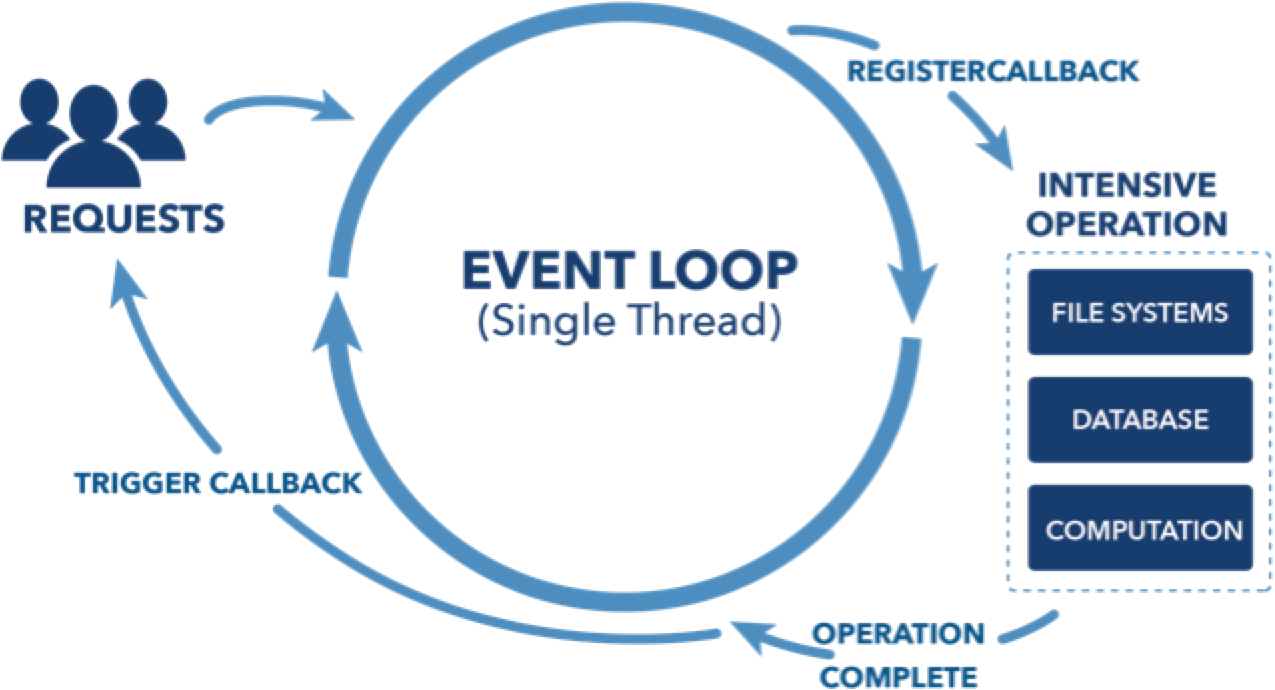
\includegraphics[width=\textwidth]{images/nodeEvent.png}
	\caption{Gestione eventi con Node.js.}
	\label{fig:nodeEvent}
\end{figure}
Bisogna però sempre tenere a mente, quando si progetta di scrivere un programma con Node.js, che questa architettura ha un effetto collaterale molto pesante; le operazioni che occupano per lungo tempo il thread in cui viene eseguito il codice (operazioni di calcolo onerose) bloccano l'interno software. Per questo motivo Node.js è assolutamente sconsigliato in caso di operazioni di calcolo complesse e nella fase di progettazione di programmi che usano questa piattaforma è sempre necessario utilizzare questa caratteristica come criterio fondamentale per la scrittura del codice.
Di seguito sono alcune delle caratteristiche importanti che rendono Node.js la prima scelta di architetti del software:
\begin{itemize}
\item \textbf{Asynchronous and Event Driven}: Tutte le API della libreria Node.js sono asincrone, ovvero non bloccanti. Significa essenzialmente che un server basato su Node non aspetta mai che un'API restituisca i dati. Il server passa all'API successiva dopo averlo chiamato ed un meccanismo di notifica di eventi consente al server di ottenere una risposta dalla precedente chiamata.
\item \textbf{Molto veloce}: Essendo costruito sul motore Javascript V8 di Google Chrome, Node.js è molto veloce nell'esecuzione del codice.
\item \textbf{Thread singolo ma altamente scalabile}: Node utilizza un singolo thread con loop di eventi. Il meccanismo degli eventi aiuta il server a rispondere in modo non bloccante e rende il server altamente scalabile rispoetto ai server tradizionali che creano thread limitati per gestire le richieste. Quindi, Node utilizza un singolo programma con thread e lo stesso programma può fornire il servizio a un numero molto più grande di richieste rispotto ai server come Apache HTTP Server.
\item \textbf{Nessun Buffering}: Le applicazioni create con node non bufferizzano mai alcun dato. Queste applicazioni generano semplicemente i dati in blocchi.
\item \textbf{Licenza}: Node è rilasciato sotto licenza MIT. 
\end{itemize}
Esiste un mondo attorno a JS composto da librerie che ne estendono le funzionalità. Stesso discorso vale per Node.js, in quanto è attiva una comunità di sviluppo che ha realizzato in questi anni molte librerie per realizzare particolari tipi di supporto (database, Network, . . . ) e Node.js offre un sistema di installazione di questi moduli che si occupa anche di eventuali dipendenze: \textit{npm}. Nei prossimi capitoli saranno analizzati alcuni progetti legati a Node.js usati nella creazione della webapp.

\subsubsection{Express Handlebars}
\label{sec:express handlebars}
Express è un framework basato su Node che offre un insieme robusto di utilità per realizzare agilmente applicazioni web single-page, multi-page e ibride. E' un framework maturo e tra le funzionalità offerte sono inclusi: il livello middleware connect, il routing, la possibilità di gestire le configurazioni dell'applicazione, un motore di templating, e molte altre funzionalità.


\subsubsection{WebSocket}
\label{sec:WebSocket}

\subsubsection{MaterialCSS}
\label{sec:materialCSS}

\subsubsection{D3js}
\label{sec:d3js}